\paragraph{Мейн функция} нулевой задачи выглядит вот так:

\begin{verbatim}
undefined8 FUN_00101170(void)

{
  int iVar1;
  char *__s1;

  __s1 = (char *)malloc(400);
  printf("%s","Hello, enter the flag:\n");
  __isoc99_scanf(&DAT_00102004,__s1);
  iVar1 = strcmp(__s1,"flag{6057f13c496ecf7fd777ceb9e79ae2 85}");
  if (iVar1 == 0) {
    printf("%s",&DAT_00102046);
  }
  else {
    printf("%s","TRY HARDER");
  }
  return 0;
}

\end{verbatim}

\paragraph{Описание}

\paragraph{}
Данный код --- это функция на языке C, реализующая проверку флага.
Опишем её по шагам:

\begin{enumerate}
    \item Выделяется память под строку:
    \begin{verbatim}
    __s1 = (char *)malloc(400);
    \end{verbatim}
    Здесь выделяются 400 байт для хранения пользовательского ввода.

    \item Печатается приглашение пользователю:
    \begin{verbatim}
    printf("%s", "Hello, enter the flag:\n");
    \end{verbatim}
    На экран выводится сообщение:
    \begin{verbatim}
    Hello, enter the flag:
    \end{verbatim}

    \item Считывается ввод:
    \begin{verbatim}
    __isoc99_scanf(&DAT_00102004, __s1);
    \end{verbatim}

    \item Введённая строка сравнивается с жёстко закодированным флагом:
    \begin{verbatim}
    iVar1 = strcmp(__s1, "flag{6057f13c496ecf7fd777ceb9e79ae285}");
    \end{verbatim}
    Если строки совпадают (iVar1 == 0), выполняется блок if, иначе --- else.

    \item Условие:
    \begin{verbatim}
    if (iVar1 == 0)
        printf("%s", &DAT_00102046);
    else
        printf("%s", "TRY HARDER");
    \end{verbatim}
    Если строка верная, выводится сообщение по адресу \&DAT\_00102046 (строка \("\)WIN\("\)), иначе выводится сообщение \("\)TRY HARDER\("\).

    \item Функция возвращает 0:
    \begin{verbatim}
    return 0;
    \end{verbatim}
\end{enumerate}

\noindent

\paragraph{Особенности}
\begin{itemize}
    \item Отсутствует освобождение памяти после \texttt{malloc} (утечка памяти);
    \item Формат ввода не позволяет вводить пробелы (если используется \%s);
    \item Сравнение производится напрямую, без шифрования или дополнительных преобразований.
\end{itemize}

\newpage

\paragraph{Тестовые запуски}

\paragraph{}
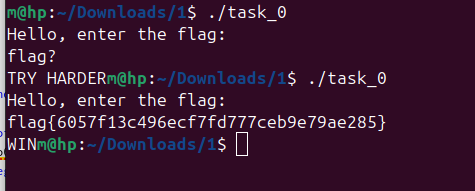
\includegraphics[width=0.7\linewidth]{static/solution_task_0}
